%!TEX root = book.teX
\chapter{ART quick start}

To use ART, all you need is a copy of the file {\tt art.jar} (and an installed Java compiler and runtime). As a quick test, make a new directory, put a copy of {\tt art.jar} in it and then type:

\begin{quote}
\begin{verbatim}
java -jar art.jar
\end{verbatim}
\end{quote}

\noindent You should see a help message, the first line of which is similar\footnote{The build-specific version number format is {\em major.minor.buildNumber.status} where {\em status} is one of {\sf white} (release version); {\sf green} (development version that passed regressions); {\sf amber} (development version that has not been regression tested); or {\sf red} (development version that failed regression testing).}
 to:
\begin{quote}
\begin{verbatim}
ART 3.0.4.GREEN usage: java -jar art.jar [options] filename
\end{verbatim}
\end{quote}
Now make a simple grammar file called {\tt first.art} as follows.
\begin{quote}
\begin{verbatim}
S ::= B 'c'
B ::= 'a' B | 'a'
\end{verbatim}
\end{quote}
and a string file {\tt first.str} containing:
\begin{quote}
\begin{verbatim}
aac
\end{verbatim}
\end{quote}
Now issue the following three commands to (i) generate a Java implementation of the parser specified in {\tt first.art}, (ii) compile the generated files {\tt ARTGLLParser.java} and {\tt ARTGLLLexer.java}, and (iii) run the compiled parser on the string in {\tt test.str} using the built in test harness 
\begin{quote}
\begin{verbatim}
java -jar art.jar first.art 
javac -classpath .;art.jar ARTGLLParser.java ARTGLLLexer.java
java -classpath .;art.jar ARTTest first.str
\end{verbatim}
\end{quote}
If all goes well, you will see no output at all\ldots\  To visualise the results of the parse, run the parser again with the {\tt -v4} option:
\begin{quote}
\begin{verbatim}
java -classpath .;art.jar ARTTest first.str -v4
\end{verbatim}
\end{quote}
You should get the following console output:
\begin{quote}
\begin{verbatim}
Accept
1: S
  2: B
    3: 'a'
    4: B
      5: 'a'
  6: 'c'
\end{verbatim}
\end{quote}
This shows that the string was accepted and presents a derivation $S\Rightarrow B c\Rightarrow a B c\Rightarrow a a c$ 

When using the {\tt -v4} option, the test harness will also have output a set of {\tt .dot} files. If you have the {\tt graphviz} programs installed on your system (see \url{http://www.graphviz.org}) then you can display derivation trees and other structures graphically. For instance, the command

\begin{quote}
\begin{verbatim}
dot -Tpdf rdt.dot > rdt.pdf
\end{verbatim}
\end{quote}

will produce a document {\tt rdt.pdf} which contains

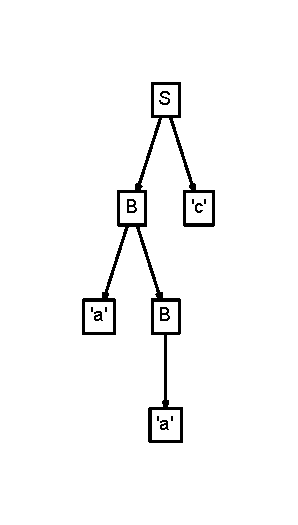
\includegraphics{firsta.pdf}

These diagrams get very large for non-trivial examples, so part of the art of interpreter development is finding small examples that help you visualise the particular feature you are working on without clutter.
\clearpage
\section{Parser generation workflow}
In this tutorial we are concentrating in the implementation of interpreters using ART's attribute grammars. The workflow for this use-case looks like this:

\vspace*{-1cm}\hspace*{-2.2cm}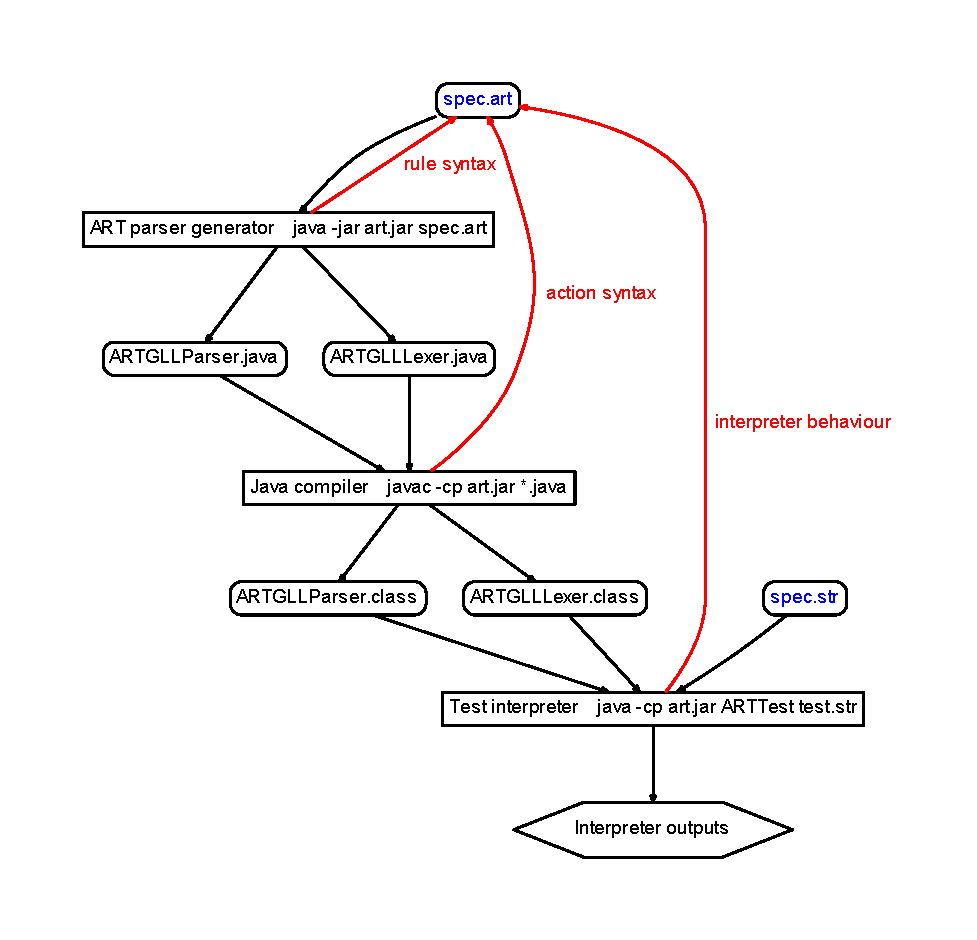
\includegraphics{artflow.pdf}\vspace*{-1cm}
Rectangular boxes represent commands; rounded boxes text files; and the hexagon box at the bottom some arbitrary behaviour, which might be the output of some translated file or the direct execution of a user program written in the language we are designing.

The black elements show the commands that we executed in the previous section; the red arrows represent the changes to the specification needed in response to three kinds of errors:
\begin{itemize}
\item ART will issue error messages if your rules have meta-syntax errors;
\item the Java compiler will issue error messages if your actions are not syntactically correct Java, or if you reference undefined identifiers;
\item your interpreter will issue syntax errors if the {\tt spec.str} file contains ill-formed constructs.
\end{itemize}

\chapter{ART basics}
We should start by making some scripts to build and run ART generated parsers. In the zip file {\tt ARTInterpreterTutorial.zip} which you can collect from Royal Holloway's Centre for Software Language Engineering website, you will find all of the examples from this tutorial along with these two simple Windows batch files:

\begin{quote}
{\sf\bfseries tst.bat}

\begin{verbatim}
java -jar art.jar %1.art 
javac -classpath .;art.jar ARTGLLParser.java ARTGLLLexer.java
java -classpath .;art.jar ARTTest %1.str %2 %3 %4 %5 %6 %7 %8 %9
\end{verbatim}
\end{quote}
and 
\begin{quote}
{\sf\bfseries run.bat}

\begin{verbatim}
java -classpath .;art.jar ARTTest %1.str %2 %3 %4 %5 %6 %7 %8 %9
\end{verbatim}
\end{quote}
We recommend that you construct the equivalent scripts for your preferred operating system shell. We shall use the {\tt tst} script form now on as a shorthand.

\section{Accepting and rejecting strings}
Create a new file {\tt second.art} with this content:
\begin{codeblock}
S ::= 'b' | 'a' X '@' (* An example grammar *)
X ::= 'x' X | # 
\end{codeblock}
Each rule begins with a nonterminal
followed by the \verb+::=+ symbol. Terminals are delimited by single quotes and $\epsilon$, the empty string, is denoted by \verb+#+. The start symbol is by default the first symbol in the specifications, and comments are delimited by {\tt (* ... *)} brackets. 

\noindent Now make a string file {\tt second.str} containing:
\begin{codeblock}
axx@
\end{codeblock}
Generate and run the parser by typing \verb+tst second -v4+ Do not add a file type. 
\begin{codeblock}
Accept
1: S
  2: a
  3: X
    4: x
    5: X
      6: x
      7: X
        8: #
  9: @
\end{codeblock}
Try changing the input by adding more \verb+x+ characters before the \verb+@+ and observe what happens.
Try removing the final \verb+@+ character and see what happens: you will see
\begin{codeblock}
1,2 Parse error: unexpected symbol follows
\end{codeblock}
The two numbers are (row, column) coordinates into the test string. The message means that the parser got as far as the symbol which starts at those coordinates; the following symbol was unexpected. Some care may be required in interpreting these messages since ART-generated parsers can in some circumstances explore putative derivations that match a long way into the source string before failing; one cannot guarantee that the coordinates in this message represent the failure of the derivation that you actually wanted. In practice, for grammars written in the style of conventional programming language grammars, the coordinates do usually indicate the error point.

\section{Using builtins}
ART is a {\em general} parser generator which places no restrictions on the form of the grammar. As such, 
it is perfectly possible to describe languages all the way down to character level, but it is often convenient to use higher-level `shrink wrapped' primitives. ART provides a family of useful builtin lexer functions which you can recognise by their leading \verb+&+ character which can be used to process things like integers (\verb+&INTEGER+), Java-style alphanumeric identifiers (\verb+&ID+) and Java-style double-quote delimited strings (\verb+&STRING_DQ+). To see builtins in action, create a file {\tt assign.art} containing

\begin{codeblock}
S ::= &ID '=' &INTEGER ';' 
\end{codeblock}
and an input file {\tt assign.str} containing
\begin{codeblock}
x = 23;
\end{codeblock}
Process the files using {\tt tst assign -v4} to generate this output
\begin{codeblock}
Accept
1: S
  2: &ID x
  3: '='
  4: &INTEGER  23
  5: ';'
\end{codeblock}

Note that the builtins are shown with their {\em lexeme} (the substring that they matched) and that the \verb+&ID+
and \verb+&INTEGER+ builtins have matched the alphanumeric identifier
and the integer. Experiment with changing the input file to have a
longer identifier or a different number. What happens if you try a
negative integer?

\section{Attributes and semantics}
Create a file {\tt abaction.art} with these contents:
\begin{codeblock}
S ::= A | B
A ::= 'a'
B ::='b'
\end{codeblock}
Now create a file containing a single {\tt a} character and run {\tt
  tst abaction -v4}.
You should see the following output
\begin{codeblock}
Accept
1: S
  2: A
    3: a
\end{codeblock}
This shows that the parser found the derivation
\[S\Rightarrow A\Rightarrow a\]
We can arrange for the grammar to announce what it has found by adding
semantic actions. In ART, an action is enclosed in braces
\verb+{ }+. Within the braces we can add any syntactically valid Java
fragment.
Modify your {\tt abaction.art} file so that it announces when it has
matched the letter {\tt a}.
\begin{codeblock}
S ::= A | B
A ::= 'a' {System.out.println("Found an a");}
B ::='b'
\end{codeblock}
Now we get this output:
\begin{codeblock}
Found an a
Accept 
1: S
  2: A
    3: a
\end{codeblock}
Change the input to {\tt b} and satisfy yourself that that the
message no longer appears.

\section{The execution order of actions}
\label{abaction}
ART first finds all the derivations of the input in the
grammar, then selects one of the (potentially infinite set of)
derivations. ART then runs an {\em attribute evaluator} which visits the
derivation tree top-down, left-to-right and executes actions as it
passes between nodes, in the order that they are written in the
grammar. By default, each node is only visited once. (You can read more about formal aspects of attribute grammars in Appendix~\ref{attribute:grammars} where you'll find that the style of evaluator we are using here is called an {\em L-attributed} evaluator in the literature.)

We now extend the grammar to match a sequence of {\tt a} characters.
\begin{codeblock}
S ::= A | B
A ::= 'a' {System.out.println("Found an a");} A | #
B ::='b'
\end{codeblock}

Run this using the input {\tt aaa} to get this output:
\begin{codeblock}
Found an a
Found an a
Found an a
Accept
1: S
  2: A
    3: a
    4: A
      5: a
      6: A
        7: a
        8: A
          9: #
\end{codeblock}
The tree has three terminal {\tt a} nodes, and the message is printed
out three times.

The deepest node in the tree is an epsilon node labeled {\tt \#}, and
it will be visited last. If we add an action to the {\tt A ::= \#}
production, we can announce that we have reached the end of the list.
\begin{codeblock}
S ::= A | B
A ::= 'a' {System.out.println("Found an a");} A | 
       {artText.println("End of list of a"); } # 
B ::='b'
\end{codeblock}
which yields
\begin{codeblock}
Found an a
Found an a
Found an a
End of list of a
Accept
1: S
  2: A
    3: a
    4: A
      5: a
      6: A
        7: a
        8: A
          9: #
\end{codeblock}
\section{The artText object}
Notice that in the previous examples we used methods {\sf System.out.println()} and {\sf artText.println()}. The {\sf artText} object provides most of the common Java text output methods, but in a way that allows messages to be captured and processed rather than being sent directly to the console. ART parsers are designed to be embedded in user applications, and it would be uncomfortable to have parser error messages sent to the console in a GUI application, in which case the artText object provides application-specific message handling.

In this tutorial we are building stand alone interpreters which should display their results on the console; it does not matter whether we use {\sf System.out} or {\sf artText} methods.

\section{Attributes}
Simply adding print statements to a grammar does not provide much
useful capability because all they can do is report where the
evaluator has got to. To make a useful translator, we need to be extract information from tree nodes and even put information into tree nodes. It turns out that so that we need to be able
to transfer information across the tree, possibly transforming it as
we go.

In an attribute grammar we define a (possibly empty) set of attributes for each nonterminal. The
actions execute in the context of a small sub-tree: each action
can `see' a single parent node and its children, but no more. The name
of the parent node will be the name of a nonterminal, and the names of
the child nodes will be the name of a nonterminal suffixed by an
integer instance number.

We have to declare our attributes by giving them a name and a type. The declaration appears in angle brackets between the defining name of a nonterminal and the {\tt ::=} symbol.
\begin{codeblock}
X <attr1:int attr2:double> ::= Y { Z1.value = X.attr2; } Z { X.attr1 = Y1.value; }

Y <value:int> ::= ...
Z <value:double> ::= ...
\end{codeblock}
In line 1, we define a production $ X ::= Y\  Z$ and declare that $X$ has two attributes called {\sf attr1} and {\sf attr2} of type {\sf int} and {\sf double} respectively. The two actions, which must be valid Java phrases, push the value of {\sf attr2} down into the {\sf value} attribute of $Z$ (an inherited attribute) and propagate the {\sf value} computed by $Y$ up into the {\sf attr1} attribute of $X$ (a synthesized attribute).

The naming conventions can be initially confusing. The attribute equations use terms written {\em nonterminalName.attributeName}. If {\em nonterminalName} corresponds exactly to the name of a nonterminal $N$ in the grammar, then it represents the left hand side of the production containing the equation whichmust be $N$. If {\em nonterminalName} $N$ is the name of a nonterminal with a numeric suffix $i$, then it refers to the $i^{th}$ instance of $N$ in this production.
\section{Computing values}
We shall now rework the grammar from the Section~\ref{abaction} so that instead of just reporting when it finds an {\tt a} character, it will {\em compute} the number of {\tt a} accepted. We do this by adding an attribute {\tt listLength} to nonterminal {\tt A}. 

For the production $A ::= \#$, we propagate the value zero to the parent. For the
 other production $S ::= A\ a$ we propagate the length returned by $A$ plus one. Finally, we then add
an action to the start symbol to print out the length. 

Make a new grammar {\tt abCount.art} which has these productions.
\begin{codeblock}
S ::= A { artText.println("List length is " + A1.listLength); } | B

A<listLength:int> ::= 'a' A { A.listLength = A1.listLength + 1; } 
                    |  # { A.listLength = 0; } 

B ::='b'
\end{codeblock}
When run on {\tt aaa} we get 
\begin{codeblock}
List length is 3
Accept
1: S
  2: A < listLength=3 >
    3: 'a'
    4: A < listLength=2 >
      5: 'a'
      6: A < listLength=1 >
        7: 'a'
        8: A < listLength=0 >
          9: #
\end{codeblock}
Notice how the textual representation of the tree includes the attribute and their values. This can be very useful for debugging. For small examples like this one, you may prefer the graphical output on the next page.

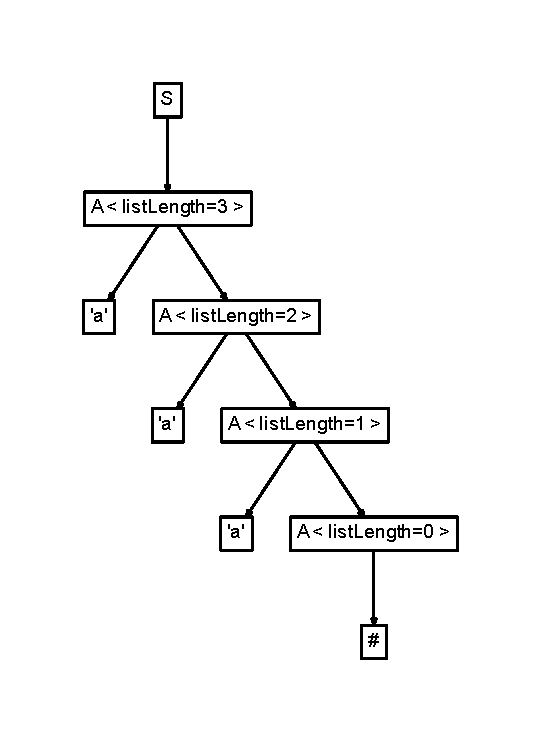
\includegraphics[scale=1]{abCount.pdf}

\chapter{The {\tt mini} languages}
In this chapter, we develop a sequence of small languages, starting with a basic calculator and building up to a language with procedures. The {\tt mini} languages are limited to simple integer variables: we are mostly focusing on the development of control flow. We shall look at more complex type systems in the next chapter.

Here is an overview of the complete sequence of language specifications.
\begin{itemize}
\item {\tt miniSyntax.art} contains just the BNF productions for a calculator
language called from a print statement.

\item {\tt miniCalc.art} is {\tt miniSyntax.art} extended with attributes and actions to
implement the semantics of a simple calculator.

\item {\tt miniAssign.art} adds a simple symbol table, an assignment statement
and variable access. The start symbol is statement which generates a
sequence of statements.

\item {\tt miniIf.art} adds an if statement and a compound statement to the
rules for statement, which reverts to being the start symbol

\item {\tt miniWhile.art} adds a while statement

\item {\tt miniCall.art} adds procedure control flow, but there are no
parameters or any sort of type system. Variables and procedures are
stored in separate hash tables.
\end{itemize}
\begin{boxedminipage}{\textwidth}
Restriction: in version 3.0 of ART, the attribute evaluator can not handle EBNF grammars, so we shall limit ourselves to BNF. BNF and EBNF have the same descriptive strength, but EBNF specifications may be more compact than equivalent BNF specifications.
\end{boxedminipage}
\clearpage
\section{{\tt miniSyntax.art} -- mini core syntax}
The heart of {\tt mini} is an arithmetic expression evaluator; programs comprise sequences of {\tt print} statements which can take sequences of strings or expressions. This is a valid {\tt miniSyntax} program
\begin{codeblock}
print("Result is ", 3+4*2);
\end{codeblock}
Here is an ART specification for the basic {\tt mini} syntax.
\begin{codeblock}
statement ::= 'print' '(' printElements ')' ';'   (* print statement *)

printElements ::= STRING_DQ | 
                  STRING_DQ ',' printElements | 
                  e0 | e0 ',' printElements  

e0 ::= e1 | 
       e1 '>'  e1 |       (* Greater than *)
       e1 '<'  e1 |       (* Less than *)
       e1 '>=' e1 |       (* Greater than or equals*)
       e1 '<=' e1 |       (* Less than or equals *)
       e1 '==' e1 |       (* Equal to *)
       e1 '!=' e1         (* Not equal to *)

e1  ::= e2 | 
        e1 '+' e2 |       (* Add *)
        e1 '-' e2         (* Subtract *)

e2  ::= e3 | 
        e2 '*' e3 |       (* Multiply *)
        e2 '/' e3 |       (* Divide *)
        e2 '%' e3         (* Mod *)

e3  ::= e4 | 
        '+' e3 |          (* Posite *)
        '-' e3            (* Negate *)

e4  ::= e5 | 
        e5 '**' e4        (* exponentiate *)

e5  ::= INTEGER |         (* Integer literal *)
        '(' e1 ')'        (* Parenthesised expression *)       

STRING_DQ ::= &STRING_DQ  
INTEGER ::= &INTEGER  
\end{codeblock}
The grammar encodes priorities and associativities for operators as follows.
\begin{quote}
\hspace*{-1.5cm}\begin{tabular}{c|ccl}
Op&Priority&Associativity&Function\\
\hline
\verb+>+&0&None&Greater than\\
\verb+<+&0&None&Less than\\
\verb+>=+&0&None&Greater than or equals\\
\verb+<=+&0&None&Less than or equals\\
\verb+==+&0&None&Equal to\\
\verb+!=+&0&None&Not equal to\\
\hline
\verb!+!&1&Left&Addition\\
\verb+-+&1&Left&Subtraction\\
\hline
\verb+*+&2&Left&Multiplication\\
\verb+/+&2&Left&Integer division\\
\verb+%+&2&Left&Integer remainder after division\\
\hline
\verb!+!&3&Left&Monadic positive value\\
\verb+-+&3&Left&Mondaic negative value\\
\hline
\verb+**+&4&Right&Integer exponention (left raised to the right$^{th}$ power)\\
\hline
\end{tabular}
\end{quote}

Notice how the builtins {\tt INTEGER} and \verb+STRING_DQ+ are wrapped in their own nonterminals. This is because terminals cannot have attributes in ART, and so if we want to extract information from a terminal we wrap it in a carrier nonterminal.

Type {\tt tst miniSyntax -v4} and you will get this output:
\begin{codeblock}
Accept
1: statement
  2: 'print'
  3: '('
  4: printElements
    5: STRING_DQ
      6: &STRING_DQ "Result is "
    7: ','
    8: printElements
      9: e0
        10: e1
          11: e1
            12: e2
              13: e3
                14: e4
                  15: e5
                    16: INTEGER
                      17: &INTEGER  3
          18: '+'
          19: e2
            20: e2
              21: e3
                22: e4
                  23: e5
                    24: INTEGER
                      25: &INTEGER 4
            26: '*'
            27: e3
              28: e4
                29: e5
                  30: INTEGER
                    31: &INTEGER 2
  32: ')'
  33: ';'
  \end{codeblock}
which corresponds to this tree

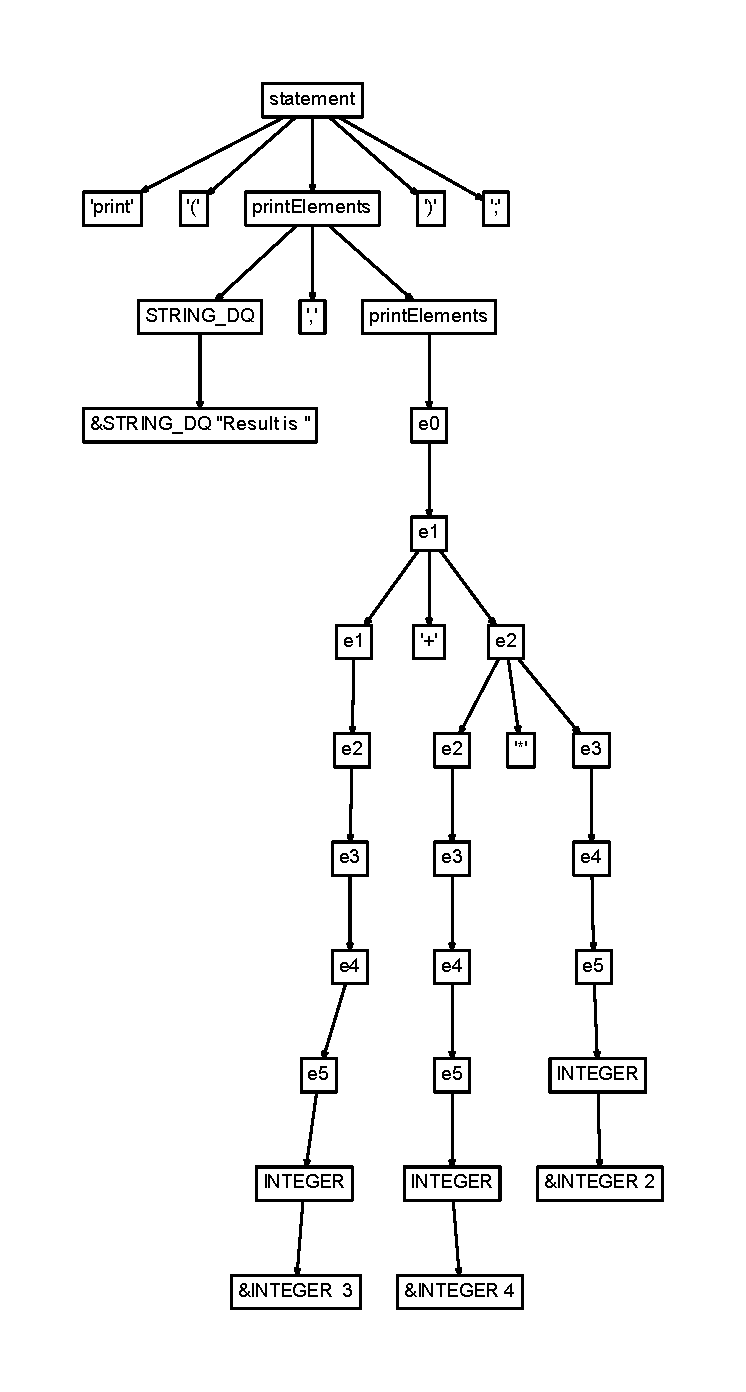
\includegraphics[scale=0.7]{miniSyntaxRDT.pdf}

\section{{\tt miniCalc} -- a calculator}
This grammar adds an attribute {\tt v} to each rule in the expression grammar, and an action which computs the value of the subexpression matched by that rule.
\begin{codeblock}
statement ::= 'print' '(' printElements ')' ';' 

printElements ::= STRING_DQ { artText.printf("%s", STRING_DQ1.v); } | 
        STRING_DQ { artText.printf("%s", STRING_DQ1.v); } ',' printElements | 
        e0 { artText.printf("%d", e01.v); } | 
        e0 { artText.printf("%d", e01.v); } ',' printElements 

e0 <v:int> ::= e1 { e0.v = e11.v; } | 
               e1 '>'  e1 { e0.v = e11.v >  e12.v ? 1 : 0; } |     
               e1 '<'  e1 { e0.v = e11.v <  e12.v ? 1 : 0; } |     
               e1 '>=' e1 { e0.v = e11.v >= e12.v ? 1 : 0; } |     
               e1 '<=' e1 { e0.v = e11.v <= e12.v ? 1 : 0; } |     
               e1 '==' e1 { e0.v = e11.v == e12.v ? 1 : 0; } |     
               e1 '!=' e1 { e0.v = e11.v != e12.v ? 1 : 0; } 

e1 <v:int>  ::= e2 { e1.v = e21.v; } | 
                e1 '+' e2 { e1.v = e11.v + e21.v; } |              
                e1 '-' e2 { e1.v = e11.v - e21.v; } 

e2  <v:int> ::= e3 { e2.v= e31.v; } | 
                e2 '*' e3 { e2.v = e21.v * e31.v; } |              
                e2 '/' e3 { e2.v = e21.v / e31.v; } |              
                e2 '%' e3 { e2.v = e21.v % e31.v; } 

e3  <v:int> ::= e4 {e3.v = e41.v; } | 
                '+' e3 {e3.v = e41.v; } |                          
                '-' e3 {e3.v = -e41.v; }                           

e4  <v:int> ::= e5 { e4.v = e51.v; } | 
                e5 '**' e4 {e4.v = (int) Math.pow(e51.v, e41.v); }  

e5  <v:int> ::= INTEGER {e5.v = INTEGER1.v; } |                     
                '(' e1 { e5.v = e11.v; } ')'                        
\end{codeblock}
As the evaluator visits each node of the tree, it performs the computation required
by that part of the syntax. The values propagate up to the {\tt print} statement via the {\tt v}
attributes. Type {\tt tst miniCalc} to run the interpreter on test string in {\tt miniCalc.str}. The test is \verb!print("Result is ", (30+4)*2, "\n");! and the output is
\begin{codeblock}
Result is 68
\end{codeblock}

\section{{\tt miniAssign} - adding variables}
The previous grammar performs computations over expressions involving
literal integers. We want to be able to add variables and an
assignment statement.

Now, at the time we write the grammar, we do not know the names of the
variables that a user might write into a program, so we cannot simply
create attributes to hold the variables. Instead, we create a {\em symbol table}, that is map
which holds bindings of values to identifiers. Assignment statements are {\em variable definitions}
which update the map with new values. A variable {\em use} on the right hand side
of an expression accesses the map to retrieve the value.

We need some directives that allow us to insert Java declarations into the generated class file. The {\sf prelude} directive takes an action with braces, and inserts it at the top of the generated source. Its main use is to add Java import directives. The {\sf support} directive takes an action in braces and inserts it at the top of the generated class. Its main use is to add class-level members to the generated class, which may effectively be treated as global variables in parser actions.

Our symbol table (called {\sf symbols}) is such a global variable. We use a sumple Java {\sf HashMap} from {\sf String} to {\sf Integer} to implement the symbol table, and make the necessary {\sf import} and member declarations using ART's {\sf prelude} and {\sf support} directives. Here is the complete specification from {\tt miniAssign.art}.
\begin{codeblock}
prelude {import java.util.HashMap;}

support { HashMap<String, Integer> symbols = new HashMap<String, Integer>(); }

statements ::= statement | statement statements  

statement ::= ID '=' e0 ';' { symbols.put(ID1.v, e01.v); } |        
              'print' '(' printElements ')' ';'                     

printElements ::= STRING_DQ { artText.printf("%s", STRING_DQ1.v); } | 
      STRING_DQ { artText.printf("%s", STRING_DQ1.v); } ',' printElements | 
      e0 { artText.printf("%d", e01.v); } | 
      e0 { artText.printf("%d", e01.v); } ',' printElements  

e0 <v:int> ::= e1 { e0.v = e11.v; } | 
               e1 '>'  e1 { e0.v = e11.v >  e12.v ? 1 : 0; } |      
               e1 '<'  e1 { e0.v = e11.v <  e12.v ? 1 : 0; } |      
               e1 '>=' e1 { e0.v = e11.v >= e12.v ? 1 : 0; } |      
               e1 '<=' e1 { e0.v = e11.v <= e12.v ? 1 : 0; } |      
               e1 '==' e1 { e0.v = e11.v == e12.v ? 1 : 0; } |      
               e1 '!=' e1 { e0.v = e11.v != e12.v ? 1 : 0; }        

e1 <v:int>  ::= e2 { e1.v = e21.v; } | 
                e1 '+' e2 { e1.v = e11.v + e21.v; } |               
                e1 '-' e2 { e1.v = e11.v - e21.v; }                 

e2  <v:int> ::= e3 { e2.v= e31.v; } | 
                e2 '*' e3 { e2.v = e21.v * e31.v; } |               
                e2 '/' e3 { e2.v = e21.v / e31.v; } |               
                e2 '%' e3 { e2.v = e21.v % e31.v; }                 

e3  <v:int> ::= e4 {e3.v = e41.v; } | 
                '+' e3 {e3.v = e41.v; } |                           
                '-' e3 {e3.v = -e41.v; }                            

e4  <v:int> ::= e5 { e4.v = e51.v; } | 
                e5 '**' e4 {e4.v = (int) Math.pow(e51.v, e41.v); }  

e5  <v:int> ::= INTEGER {e5.v = INTEGER1.v; } |                     
                ID { e5.v = symbols.get(ID1.v); } |                 
                '(' e1 { e5.v = e11.v; } ')'                        
\end{codeblock}

Try running the parser using the command {\tt tst miniAssign -v4} on this input
\begin{codeblock}
temp = 3+4*2;
print("Initial result is ", temp, "\n");
temp = temp + 1;
print("Final result is ", temp, "\n");
\end{codeblock}
generating this result
\begin{codeblock}
Initial result is 11
Final result is 12
\end{codeblock}

You might like to try these self-assessment exercises.

\begin{enumerate}
\item Add left-associative left shift and right shift operators (\verb+<<+ and
  \verb+>>+) to the {\tt miniAssign} grammar with priority between addition and relational operators.

\item Add a check action to the rule for \verb+e5+ which catches the
  use of an undefined variable.
\item In fact, the approach is rather fragile. If we try to access an
undefined variable, then the semantic action in the rule
\verb+e5 ::= ID+ will yield a {\tt null} value. Try changing the input
to generate this error.
\end{enumerate}
\clearpage
\section{Interlude -- delayed attributes and flow control}
In the interpreters we have written so far, the parser builds a derivation tree and then the attribute evaluator makes a single top-down, left-to-right traversal of that derivation tree, executing the actions as it goes.

This approach is sufficient for simple linear programs, but we might want to execute, say, a loop in which the part of the derivation tree corresponding to the loop's body is executed multiple times.

ART's mechanism for supporting non-linear control flow is the {\em delayed} attribute. If we annotate a right hand side nonterminal instance with a `less than' character \verb+<+, then the evaluator will {\em not descend} into the corresponding subtree. Instead, a reference to the subtree called its {\em handle} will be stored in an attribute of the left hand side nonterminal. The attribute evaluator function is user-accessible, and that means that at a point of our choosing we can invoke the evaluator on the stored handle.

We introduce delayed attributes by implementing an {\sf if} statement. Create a new file {\tt delay.art} containing:
\begin{codeblock}
S ::= 'if' P 'then' A 
P ::= 'true' | 'false'  
A ::= 'print' 
\end{codeblock}
The language of this grammar is the set of two strings \begin{quote}\{ \verb+if true then print+, \verb+if false then print+ \}\end{quote} 
Create a parser for {\tt delay} and use the {\tt tst} script to it to parse both inputs, verifying that the derivation tree for the first element is:
\begin{codeblock}
Accept
1: S
  2: if
  3: P
    4: true
  5: then
  6: A
    7: print
\end{codeblock}
Now expand the grammar with attributes and actions as follows:
\begin{codeblock}
S ::= 'if' P 'then' A 
P<v:boolean> ::= 'true' {P.v = true;} | 'false' {P.v = false;}  
A ::= 'print' {artText.println("Printed");}  
\end{codeblock}
Note that we have not yet added a delayed attribute, so this interpreter will directly execute all of the action. Thus, when run with the input \verb+if true then print+, we get this output
\begin{codeblock}
Printed
1: S
  2: if
  3: P
    4: true
  5: then
  6: A
    7: print
\end{codeblock}
but unfortunately, we get almost the same output with the other input\ldots
\begin{codeblock}
Printed
1: S
  2: if
  3: P
    4: false
  5: then
  6: A
    7: print
\end{codeblock}
We shall now add a delayed attribute to the instance of A, and use the result of P to decide whether to evaluate A, thus building an interpreter for {\tt if} statements.
\begin{codeblock}
S<dummy:int> ::= 'if' P 'then' A< { if (P1.v) artEvaluate(S.A1, A1);}  
P<v:boolean> ::= 'true' {P.v = true;} | 'false' {P.v = false;}  
A ::= 'print' {artText.println("Printed");}  
\end{codeblock}
There are two new things happening here. 

Firstly, the \verb+<+ annotation on the instance of {\tt A} delays the evaluation and causes the handle of the derivation subtree rooted on the instance of A to be loaded into an attribute called {\tt S.A1}.

Secondly, within the semantic action, we look at the value returned by P, and only evaluate {\tt A} if that value is true. Evaluation means, call the function {\tt artEvaluate()} on the contents of the attribute {\tt S.A1}. In general, we need to supply attributes for the instance of {\tt A} to work with (even though this particular nonterminal has no attributes) and ART automatically creates such  block, again with the instance name of the delayed nonterminal. Hence, the full call is \verb+artEvaluate(S.A1, A1);+


Look closely at the tree too. The tree is built by the `automatic' outer instance of the evaluator function. Since it does not descend into {\tt A}, the subtree for {\tt A} is truncated and as a result node 7 from the undelayed tree does not appear.

Here is the output for {\tt if true then print}
\begin{codeblock}
Printed
Accept
1: S < dummy=0 >
  2: 'if'
  3: P < v=true >
    4: 'true'
  5: 'then'
  6: A
\end{codeblock}
and here is the output for {\tt if false then print}
\begin{codeblock}
Accept
1: S < dummy=0 >
  2: 'if'
  3: P < v=false >
    4: 'false'
  5: 'then'
  6: A
  \end{codeblock}

As we might hope, the word {\tt Printed} appears for the {\tt if true} variant and not for the {\tt if false}.
\clearpage
\section{{\tt miniIf} -- adding conditional flow control}
In Mini, the only available type is {\tt int}. We shall use an integer value of zero to represent false and any other integer value to represent true, just as in ANSI C.
 
We need to take some care with the syntax of the {\tt if then else} statement\,---\,we only have BNF available so we make a rule called {\tt elseOpt} which matches either $\epsilon$ or {\tt else ...}. We then delay evaluation of both {\tt statement} and {\tt elseOpt}, placing the evaluation under the control of the value computed by {\tt e0}.
\begin{codeblock}
prelude {import java.util.HashMap;}

support { HashMap<String, Integer> symbols = new HashMap<String, Integer>(); }

statement ::= ID '=' e0 ';' { symbols.put(ID1.v, e01.v); } |   (* assignment *)

              'if' e0 'then' statement< elseOpt<           (* if statement *)
              { if (e01.v != 0) 
                  artEvaluate(statement.statement1, statement1); 
                else
                  artEvaluate(statement.elseOpt1, elseOpt1);  
              } |
              
              'print' '(' printElements ')' ';' |             

              '{' statements '}'                                 

elseOpt ::= 'else' statement | #     

statements ::= statement | statement statements  

printElements ::= STRING_DQ { artText.printf("%s", STRING_DQ1.v); } | 
  STRING_DQ { artText.printf("%s", STRING_DQ1.v); } ',' printElements | 
  e0 { artText.printf("%d", e01.v); } | e0 { artText.printf("%d", e01.v); } 
     ',' printElements  

e0 <v:int> ::= e1 { e0.v = e11.v; } | 
   e1 '>'  e1 { e0.v = e11.v >  e12.v ? 1 : 0; } |       (* Greater than *)
   e1 '<'  e1 { e0.v = e11.v <  e12.v ? 1 : 0; } |       (* Less than *)
   e1 '>=' e1 { e0.v = e11.v >= e12.v ? 1 : 0; } |       (* Greater than or equals*)
   e1 '<=' e1 { e0.v = e11.v <= e12.v ? 1 : 0; } |       (* Less than or equals *)
   e1 '==' e1 { e0.v = e11.v == e12.v ? 1 : 0; } |       (* Equal to *)
   e1 '!=' e1 { e0.v = e11.v != e12.v ? 1 : 0; }         (* Not equal to *)

e1 <v:int>  ::= e2 { e1.v = e21.v; } | 
   e1 '+' e2 { e1.v = e11.v + e21.v; } |                (* Add *)
   e1 '-' e2 { e1.v = e11.v - e21.v; }                  (* Subtract *)

e2  <v:int> ::= e3 { e2.v= e31.v; } | 
   e2 '*' e3 { e2.v = e21.v * e31.v; } |                (* Multiply *)
   e2 '/' e3 { e2.v = e21.v / e31.v; } |                (* Divide *)
   e2 '%' e3 { e2.v = e21.v % e31.v; }                  (* Mod *)

e3  <v:int> ::= e4 {e3.v = e41.v; } | 
   '+' e3 {e3.v = e41.v; } |                            (* Posite *)
   '-' e3 {e3.v = -e41.v; }                             (* Negate *)

e4  <v:int> ::= e5 { e4.v = e51.v; } | 
   e5 '**' e4 {e4.v = (int) Math.pow(e51.v, e41.v); }   (* exponentiate *)

e5  <v:int> ::= INTEGER {e5.v = INTEGER1.v; } |         (* Integer literal *)
   ID { e5.v = symbols.get(ID1.v); } |                  (* Variable access *)
   '(' e1 { e5.v = e11.v; } ')'                         (* do-first *)
       
ID <leftExtent:int rightExtent:int lexeme:String v:String> ::= 
  &ID {ID.lexeme = artLexeme(ID.leftExtent, ID.rightExtent); 
       ID.v = artLexemeAsID(ID.leftExtent, ID.rightExtent); }  

INTEGER <leftExtent:int rightExtent:int lexeme:String v:int> ::= 
  &INTEGER {INTEGER.lexeme = artLexeme(INTEGER.leftExtent, INTEGER.rightExtent); 
     INTEGER.v = artLexemeAsInteger(INTEGER.leftExtent, INTEGER.rightExtent); }  

STRING_DQ <leftExtent:int rightExtent:int lexeme:String v:String> ::= 
  &STRING_DQ {STRING_DQ.lexeme = 
                  artLexeme(STRING_DQ.leftExtent, STRING_DQ.rightExtent); 
  STRING_DQ.v = artLexemeAsString(STRING_DQ.leftExtent, STRING_DQ.rightExtent); }  
\end{codeblock}
\clearpage  
\section{{\tt miniWhile} -- adding loops}
The specification {\tt miniwhile.art} further extends Mini with a {\tt while} loop. Here is the key addition:
\begin{codeblock}
              'while' e0< 'do' statement<          (* while statement *)
              { artEvaluate(statement.e01, e01); 
                while (e01.v != 0) { 
                  artEvaluate(statement.statement1, statement1); 
                  artEvaluate(statement.e01, e01); 
                } 
              } | 
\end{codeblock}

The syntactic structure is very similar to an {\tt if} statement, but we need to implement the actions with care. We make an initial evaluation of {\tt e0},	 and then loop over the body and a re-evaluation of {\tt e0} as long as the returned value is non-zero.

This is the first time we have seen a sub-tree evaluated more than once. The tree is a purely syntactic structure, and our attribute schemes (even these higher-order delayed attributes) do not allow us to change the tree. Therefore, the only way that we can see any variation in the evaluation of a sub-tree results from side effects. In this case, the relevant side effects are the updating of values in the symbol table as a result of assignments.

When run on this input
\begin{codeblock}
{
x = 3;
while x > 0 do { print("x is ", x, "\n"); x = x -1; }
}
\end{codeblock}
We get this output
\begin{codeblock}
x is 3
x is 2
x is 1
\end{codeblock}
\clearpage
\section{{\tt miniCall} - adding procedures}
Attributes are only locally visible, and that is true for delayed attributes too. Procedure call is non-local in the sense that we define procedures (functions, subroutines, methods, call them what you will) in one part of a program, and we call the code from potentially many places in the program.  

To connect calls to their procedure definitions, therefore, we need to be able to propagate information across the tree, in much the same way that we need to connect assignment statements to their corresponding variable usages. As we saw in the previous lab, we can do this by creating a map between identifiers and values. We can use the same idea to connect the names of procedures to their code bodies.

In a real compiler we often use a single hierarchical name space to handle variables and procedure names. To keep things simple in minicall.art, we have two independent maps, one for the variable names and one for the procedures. This allows us have a map from identifiers to integers to support assignments and variable usages, and another map from identifiers to tree nodes to support procedure definition an call. As a further simplification, we use explicit syntax to flag procedure calls with a {\tt call} keyword.

{\tt minicall.art} extends {\tt miniwhile.art} with these productions:
\begin{codeblock}
support {HashMap<String, artTT> procedures = new HashMap<String, artTT>();}

statement ::=  'procedure' ID statement< 
                       { procedures.put(ID1.v, statement.statement1); } |
              
           'call' ID ';' { artEvaluate(procedures.get(ID1.v), null); } |
\end{codeblock}
If we run this extended grammar with the input
\begin{codeblock}
{
procedure sub { print("Hello from a procedure\n"); }
x = 3;
while x > 0 do { print("x is ", x, "\n"); x = x -1; }
call sub;
}
\end{codeblock}
we get this output
\begin{codeblock}
x is 3
x is 2
x is 1
Hello from a procedure
\end{codeblock}
This implementation is quite limited. Apart from the syntactic clumsiness, our procedures have no parameters or return values.

\chapter{Cava\,--\,neither C nor Java}
In the {\tt mini} languages we have concentrated on the development of control flow statements. This is because adding a full type system to a language can become quite onerous: for instance, in Java there are four integer types and two floating point types, each of which is available as a primitive type or` as a `boxed' object type. All of the arithmetic operators can take a pair of any of these types along with the {\tt char} and {\tt Character} types. So, even before we look at arrays and classes there is a very broad set of operations that must be specified.

{\em Cava} is a language that uses C/Java style control flow operations, but which has a dynamic type system, and this allows us to offload much of the complexity onto a very regular set of Java classes.

\section{{\sf ARTValue} -- a built in dynamic type and operation system}
In a strictly-typed dynamic language, every value carries its type around with it and type compatibility is checked at runtime. The ART system comes with a package called {\tt artvalue} that contains carrier classes for all of the common elementary types along with constructors for compounds such as arrays and sets. All of these classes are subclasses of {\sf ARTValue} which contains a method for each operation (such as {\sf add(), subtract(), get()} and {\sf put()}) and for each coercion {\sf to\_{\em type}()} where {\sf\em type} is one of the {\sf ARTValue} subtypes. In the {\sf ARTValue} class, each of these methods produces an error message. The idea is that each for of the {\sf ARTValue{\em type}} subtypes, appropriate operation methods are overloaded with the relevant underlying operation; if a user tries to perform an unsupported operation then the method in the {\sf ARTValue} superclass will issue a runtime error.

Here is an excerpt from {\sf ARTValue.java}
\begin{codeblock}
package uk.ac.rhul.cs.csle.artvalue;

public abstract class ARTValue {
...
  private void errorOp(String op, ARTValue r) {
    System.err.println(
      "Value class " + strip(this.getClass().toString()) + 
      " does not provide operation " + op + " with class " + 
      strip(r.getClass().toString()) + "\n");
  }
...
  public ARTValue gt(ARTValue r) {
    errorOp("gt", r);
    return null;
  }
...
  public ARTValue mul(ARTValue r) {
    errorOp("mul", r);
    return null;
  }
...
  public int to_int() {
    errorOp("to_int");
    return 0;
  }

  public double to_double() {
    errorOp("to_double");
    return 0.0;
  }
...
}
\end{codeblock}
and the corresponding excerpts from {\sf ARTValueInteger} with overloads. 
\begin{codeblock}
package uk.ac.rhul.cs.csle.artvalue;

public class ARTValueInteger extends ARTValue {
  int l = 0;

  public ARTValueInteger(int l) {
    this.l = l;
  }
...
  @Override
  public ARTValue gt(ARTValue r) {
    return new ARTValueBoolean(l > r.to_int());
  }
...
  @Override
  public ARTValue mul(ARTValue r) {
    return new ARTValueInteger(l * r.to_int());
  }
...
  @Override
  public int to_int() {
    return l;
  }

  @Override
  public double to_double() {
    return l;
  }
...
}
\end{codeblock}
Note that all of the methods take arguments of type {\sf ARTValue} and return an {\sf ARTValue}. This will allow us to construct a grammar which has a uniform, type-independent syntax and effectively delegate all of the complexity of the type system to the code in the {\sf artvalue} package. Of course, these classes can also be used with a statically typed language. This is particularly useful when prototyping static languages because the dynamic checking will catch any missing checks for you rather than generating potentially subtle and hard-to-find errors.

\section{Implementing nested scope rules}
The mini languages have a single scope region, and as a result the procedures in {\tt miniCall} cannot have their own local variables or even parameters (which are a form of local variable). Most modern languages make use of statically resolved nested scope regions: each function or procedure has its own scope region, and in languages such as Java, the control expression and body of a {\sf for} loop also constitutes a local scope\,---\,this is what allows local declaration of induction variables in loops of the form
\begin{quote}
\begin{verbatim}
for (int i = 0; i < 10; i++) print(i);
\end{verbatim}
\end{quote}
One way of implementing nested scopes is to associate a map with each scope region, and to link the maps into a tree in which the outermost scope map is the root, and each new scope is a child of its enclosing scope. The {\sf artvalue} package provides a type constructor class {\sf ARTValueMapHierarchy} which implements this functionality. Each instance contains a Java {\sf HashMap} and a link to the parent {\sf ARTValueMapHoerarchy} element. The root node has a {\sf null} parent link. The {\sf declare()} method is used to create a binding in the target map. It is an error to {\sf declare()} the same key twice in a particular map. The {\sf put()} and {\sf get()} methods work just as for the normal Java {\sf Map} class except that the chain of scopes back to th root will be searched, and the first instance of the key will be used.

\section{The Cava specification}

Below is a complete Cava interpreter written as an ART attribute grammar. It has many similarities to {\tt miniCall}. The same set of operators is supported, but they operate on elements of {\sf ARTValue} rather than {\sf int}. Production {\sf e5} has been expanded to support many more kinds of literals, with associated calls to constructors of {\sf ARTValue} types. The control flow syntax has been changed to use C/Java style, and a {\sf for} loop has been added. The two symbol tables in {\tt miniCall} have been replaced by a single {\sf ARTValueMapHierarchy}, and functions are implemented via a {\sf ARTValueFunction} which includes methods for managing formal and actual parameter loading.

\subsection{Whitespace handling}
In all of the examples up until now we have used ART's default whitespace handling conventions. ART provides a {\sf whitespace} directive which can be used to declare a set of whitespace conventions. In the Cava specification, we define whitespace to include the default (newlines, tabs, space characters and so on) along with the two Java/C style comment conventions: \verb+//+ to line end and \verb+/*  */+ brackets using the builtins \verb+&WHITESPACE+, \verb+&COMMENT_LINE_C+ and \verb+&COMMENT_BLOCK_C+ respectively.

\begin{codeblock}
prelude 
{ import java.util.Map;
  import java.util.LinkedList;
  import java.util.HashMap;
  import java.util.LinkedHashMap;
  import uk.ac.rhul.cs.csle.artvalue.*; }

whitespace &WHITESPACE
whitespace &COMMENT_BLOCK_C
whitespace &COMMENT_LINE_C 

support 
{ ARTValueMapHierarchy<String, ARTValue> refs = 
     new ARTValueMapHierarchy<String, ARTValue>(); 
  final ARTValueVoid VOID = new ARTValueVoid(); 
  final ARTValueInteger ZERO = new ARTValueInteger(0); 
  final ARTValueBoolean TRUE = new ARTValueBoolean(true); 
  final ARTValueBoolean FALSE = new ARTValueBoolean(false); }

text ::= statements

statements ::= statement | statement statements  

statement ::= expr ';' 

  | 'if' '(' expr ')' statement< elseOpt<     (* if statement *)
  { if (expr1.v.to_boolean()) artEvaluate(statement.statement1, statement1); 
  else artEvaluate(statement.elseOpt1, elseOpt1); }     

  | 'while' '(' expr< ')' statement<          (* while statement *)
  { artEvaluate(statement.expr1, expr1); 
    while (expr1.v.to_boolean()) { 
      artEvaluate(statement.statement1, statement1); 
      artEvaluate(statement.expr1, expr1); } }  

  | 'for' '(' expr< ';' expr< ';' expr< ')' statement<  (* while statement *)
  { artEvaluate(statement.expr1, expr1);        // perform initialisation
    artEvaluate(statement.expr2, expr2);        // perform first test
    while (expr2.v.to_boolean()) { 
      artEvaluate(statement.statement1, statement1); 
      artEvaluate(statement.expr3, expr3);      // perform increment 
      artEvaluate(statement.expr2, expr2); } }  // perform test       

  | 'print' '(' printElements ')' ';'         (* print statement *)
  
  | 'println' '(' printElements ')' ';' { artText.print("\\n"); } (* println statement *)
  
  | '{' statements '}'              (* compound statement *)

  | 'ref' ID '(' { formals1.v = new LinkedHashMap<String, ARTValue>(); } formals ')'
    '{' statements< '}'
    { refs.declare(ID1.v, new ARTValueFunction(statement.statements1, formals1.v)); }   

elseOpt ::= 'else' statement | #     

printElements ::= 
  # 
  | expr { artText.print(expr1.v.to_String()); } 
  | expr { artText.print(expr1.v.to_String()); } ',' printElements  

formals<v:LinkedHashMap<String, ARTValue>> ::= 
  # 
  | ID { formals.v.put(ID1.v, ZERO); }          
  | ID { formals.v.put(ID1.v, ZERO); formals1.v = formals.v; } ',' formals
  | ID '=' e0 { formals.v.put(ID1.v, e01.v); } 
  | ID '=' e0 { formals.v.put(ID1.v, e01.v); formals1.v = formals.v; } ',' formals

expr <v:ARTValue> ::= 
  e0 { expr.v = e01.v; } 
  | ID '=' expr { refs.put(ID1.v, expr1.v); expr.v = expr1.v; }           (* Assignment *)
  | 'ref' ID { expr.v = ZERO; refs.declare(ID1.v, expr.v); }    (* Declaration standard initialisation *)
  | 'ref' ID '=' expr { expr.v = expr1.v; refs.declare(ID1.v, expr1.v); } (* Declaration *)


e0 <v:ARTValue> ::= 
  e1 { e0.v = e11.v; }  
  | e1 '>'  e1 { e0.v = e11.v.gt(e12.v); }      (* Greater than *)
  | e1 '<'  e1 { e0.v = e11.v.lt(e12.v); }      (* Less than *)
  | e1 '>=' e1 { e0.v = e11.v.ge(e12.v); }      (* Greater than or equals*)
  | e1 '<=' e1 { e0.v = e11.v.le(e12.v); }      (* Less than or equals *)
  | e1 '==' e1 { e0.v = e11.v.eq(e12.v); }      (* Equal to *)
  | e1 '!=' e1 { e0.v = e11.v.ne(e12.v); }      (* Not equal to *)

e1 <v:ARTValue> ::= 
  e2 { e1.v = e21.v; }  
  | e1 '+' e2 { e1.v = e11.v.add(e21.v); }      (* Add *)
  | e1 '-' e2 { e1.v = e11.v.sub(e21.v); }      (* Subtract *)

e2 <v:ARTValue> ::= 
  e3 { e2.v= e31.v; }   
  | e2 ':' e3 { e2.v = e21.v.cat(e31.v); }      (* Concatenation *)
  | e2 '*' e3 { e2.v = e21.v.mul(e31.v); }      (* Multiply *)
  | e2 '/' e3 { e2.v = e21.v.div(e31.v); }      (* Divide *)
  | e2 '%' e3 { e2.v = e21.v.mod(e31.v); }      (* Mod *)

e3 <v:ARTValue> ::= 
  e4 {e3.v = e41.v; }   
  | '+' e3 {e3.v = e41.v.pos(); }      (* Posite *)
  | '-' e3 {e3.v = e41.v.neg(); }      (* Negate *)

e4 <v:ARTValue> ::= 
  e5 { e4.v = e51.v; }  
  | e5 '**' e4 { e4.v = e51.v.exp(e41.v); }      (* Exponentiate *)

e5 <v:ARTValue r:ARTValueMapHierarchy<String, ARTValue> > ::= 
  INTEGER {e5.v = INTEGER1.v; }      (* Integer literal *)
  | REAL {e5.v = REAL1.v; }            (* Real literal *)
  | STRING_SQ {e5.v = STRING_SQ1.v; }  (* Character literal *)
  | STRING_DQ {e5.v = STRING_DQ1.v; }  (* String literal *)
  | 'true' {e5.v = TRUE;}    (* Boolean literal true *) 
  | 'false' {e5.v = FALSE;}            (* Boolean literal false *)
  | '(' expr { e5.v = expr1.v; } ')'   (* Parenthesised expression *)
  | ID { e5.v = refs.get(ID1.v); }     (* Variable access *)
  | ID '('            (* Call *) 
  { e5.r = refs; 
  refs = new ARTValueMapHierarchy<String, ARTValue>(refs, refs.get(ID1.v).getParameters()); } 
  actuals ')' { artEvaluate(refs.get(ID1.v).getBody(), null); e5.v = VOID; refs = e5.r; }

actuals ::= 
  { unnamedActuals1.v = new LinkedList<ARTValue>(); } 
  unnamedActuals { refs.loadUnnamedActuals(unnamedActuals1.v); }
  | { unnamedActuals1.v = new LinkedList<ARTValue>(); } 
  unnamedActuals { refs.loadUnnamedActuals(unnamedActuals1.v); }  ',' namedActuals 
  |  namedActuals

unnamedActuals<v:LinkedList<ARTValue>> ::= 
  # 
  | e1 { unnamedActuals.v.add(e11.v); } 
  | e1 { unnamedActuals.v.add(e11.v); } ',' 
  { unnamedActuals1.v = unnamedActuals.v; } unnamedActuals

namedActuals ::= 
  # 
  | ID '=' e1 { refs.put(ID1.v, e11.v); } 
  | ID '=' e1 { refs.put(ID1.v, e11.v); } ',' namedActuals

(* Lexical syntax *)
ID <leftExtent:int rightExtent:int lexeme:String v:String> ::= 
  &ID {ID.lexeme = artLexeme(ID.leftExtent, ID.rightExtent); 
  ID.v = artLexemeAsID(ID.leftExtent, ID.rightExtent); }  

INTEGER <leftExtent:int rightExtent:int lexeme:String v:ARTValueInteger> ::= 
  &INTEGER 
  { INTEGER.lexeme = artLexeme(INTEGER.leftExtent, INTEGER.rightExtent); 
  INTEGER.v = new ARTValueInteger(artLexemeAsInteger(INTEGER.leftExtent, INTEGER.rightExtent)); }  

REAL <leftExtent:int rightExtent:int lexeme:String v:ARTValueReal> ::= 
  &REAL 
  { REAL.lexeme = artLexeme(REAL.leftExtent, REAL.rightExtent); 
  REAL.v = new ARTValueReal(artLexemeAsReal(REAL.leftExtent, REAL.rightExtent)); }  

STRING_SQ <leftExtent:int rightExtent:int lexeme:String v:ARTValueChar> ::= 
  &STRING_SQ 
 { STRING_SQ.lexeme = artLexeme(STRING_SQ.leftExtent, STRING_SQ.rightExtent); 
  STRING_SQ.v = 
  new ARTValueChar(artLexemeAsString(STRING_SQ.leftExtent, STRING_SQ.rightExtent).charAt(0)); }  

STRING_DQ <leftExtent:int rightExtent:int lexeme:String v:ARTValueString> ::= 
  &STRING_DQ 
  { STRING_DQ.lexeme = artLexeme(STRING_DQ.leftExtent, STRING_DQ.rightExtent); 
  STRING_DQ.v = 
  new ARTValueString(artLexemeAsString(STRING_DQ.leftExtent, STRING_DQ.rightExtent)); }  
\end{codeblock}


\chapter{{\tt miniMusic} -- a domain specific language for playing melodies}
We complete this tutorial by returning to the {\tt mini} series and creating a Domain Specific Language for playing music. Java has a standard API for handling MIDI instruments and also includes a synthesizer. You can learn about the MIDI implementation by following Oracle's tutorial at \url{https://docs.oracle.com/javase/tutorial/sound/overview-MIDI.html}
\section{The {\tt miniMusic} architecture}
The Java MIDI API classes are extremely rich, and a detailed understanding of their features requires much reading, and a working knowledge of the way MIDI instruments interact. So as to offer a simple way in to Java MIDI, we have written a class {\sf MiniMusicPlayer} which allows you to play notes and chords in real time at a user-defined tempo. The facilities are extremely limited compared to the underlying API, but the class forms a simple first example. 

The {\tt miniMusic} language is a Domain Specific extension to {\tt miniCall} which connects to the {\tt MiniMusicPlayer} classes; essentially the complex semantic actions that {\em might} have been embedded directly into the grammar have been factored out into a separate Java class.
\begin{center}
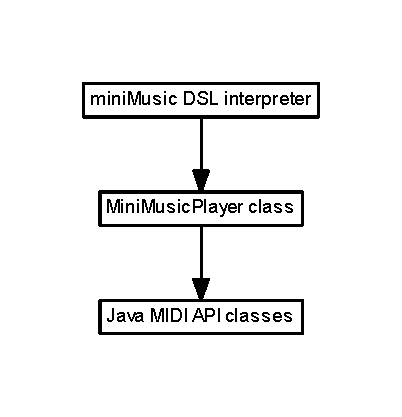
\includegraphics{miniMusicLayers.pdf}
\end{center}
\section{{\tt miniMusic} programs}
The syntax of {\tt miniMusic} is essentially that of {\tt miniCall}, except that a procedure is now referred to as a {\sf melody} and melodies are activated with a {\sf play} command. The language
accepts the standard names for notes, along with some chord designators. The note name {\sf C} designates middle C, {\sf C+} denotes the C one octave above middle C and {\sf C-} the note one octave below middle C. Multiple {\sf +} and {\sf -} characters may be used to shift notes, up to the limit of the MIDI keyboard standard. You may also attach a {\em chord suffix} such as {\sf M} for major and {\sf m} for minor, in which case a full chord will be played rather than just a single note.

Here is an example program which does some meaningless computation as well as playing a tune.
\begin{codeblock}
melody sanctuary {

D+ C+ B+M G F G m D m7
}

x = 3;
while x > 0 do { print("x is ", x, "\n"); x = x -1; }

play sanctuary;
\end{codeblock}

You can try out the {\tt miniMusic} language in the usual way by typing {\tt tst miniMusic}.\\[2ex]

\noindent\begin{boxedminipage}{\textwidth}
Restriction: in the versions of Java current in April 2017, there is a bug in the MIDI API for some operating systems which will generate this spurious error message. It may be safely ignored.
\begin{verbatim}
[Ljavax.sound.midi.MidiDevice$Info;@7291c18f
Apr 03, 2017 11:23:49 AM 
java.util.prefs.WindowsPreferences <init>
WARNING: Could not open/create prefs root node 
Software\JavaSoft\Prefs at root 0x80000002. 
Windows RegCreateKeyEx(...) returned error code 5.
\end{verbatim}
\end{boxedminipage}

\section{The {\tt miniMusic} attribute grammar}
\begin{codeblock}
prelude { import java.util.HashMap; import uk.ac.rhul.cs.csle.artmusic.*; }

support { 
HashMap<String, Integer> variables = new HashMap<String, Integer>(); 
HashMap<String, ARTGLLRDTHandle> melodies = new HashMap<String, ARTGLLRDTHandle>(); 
ARTMiniMusicPlayer mp = new ARTMiniMusicPlayer();
}

whitespace &WHITESPACE
whitespace &COMMENT_NEST_ART 
whitespace &COMMENT_LINE_C 

statements ::= statement | statement statements  

statement ::= ID '=' e0 ';' { variables.put(ID1.v, e01.v); } |     (* assignment *)

    'if' e0 'then' statement< elseOpt<         (* if statement *)
    { if (e01.v != 0) 
        artEvaluate(statement.statement1, statement1); 
      else
        artEvaluate(statement.elseOpt1, elseOpt1);  
    } |
    
    'while' e0< 'do' statement<      (* while statement *)
    { artEvaluate(statement.e01, e01); 
      while (e01.v != 0) { 
        artEvaluate(statement.statement1, statement1); 
        artEvaluate(statement.e01, e01); 
      } 
    } | 

    'print' '(' printElements ')' ';' |         (* print statement *)

    'melody' ID statement< { melodies.put(ID1.v, statement.statement1); } |
    'play' ID ';' 
      { if (!melodies.containsKey(ID1.v))
          artText.println(ARTTextLevel.WARNING, 
            "ignoring request to play undefined melody: " + ID1.v);
        else
          artEvaluate(melodies.get(ID1.v), null); 
      } |

    '{' statements '}' |              (* compound statement *)

    bpm | defaultOctave | note | chord |  rest

elseOpt ::= 'else' statement | #     

bpm ::= 'bpm' INTEGER { mp.setBpm(INTEGER1.v); }

beatRatio ::= 'beatRatio' REAL { mp.setBeatRatio(REAL1.v); }

defaultOctave ::= 'defaultOctave' INTEGER 
 { if (INTEGER1.v < 0 || INTEGER1.v > 10) 
     artText.println(ARTTextLevel.WARNING, 
       "ignoring illegal MIDI octave number " + INTEGER1.v);
    else
      mp.setDefaultOctave(INTEGER1.v); 
 }

note ::= simpleNote chordMode { mp.playChord(simpleNote1.v.trim(), chordMode1.v ); } | 
         
         simpleNote shifters chordMode 
         { mp.playChord(simpleNote1.v.trim(), mp.getDefaultOctave() + shifters1.v, chordMode1.v); } | 
         
         simpleNote INTEGER chordMode { mp.playChord(simpleNote1.v.trim(), 
          INTEGER1.v, chordMode1.v); }

chordMode <v:ARTChord> ::= # { chordMode.v = ARTChord.NONE; } | 
       'm' { chordMode.v = ARTChord.MINOR; } | 
       'm7' { chordMode.v = ARTChord.MINOR7; } | 
       'M' { chordMode.v = ARTChord.MAJOR; } | 
       'M7' { chordMode.v = ARTChord.MAJOR7; }

simpleNote<leftExtent:int rightExtent:int v:String> ::= 
  simpleNoteLexeme 
    { simpleNote.v = artLexeme(simpleNote.leftExtent, simpleNote.rightExtent).trim(); }

simpleNoteLexeme ::= 'A' | 'A#' | 'Bb' | 'B' | 'C' | 'C#' | 'Db' | 'D' | 
           'D#' | 'Eb' | 'E' | 'F' | 'F#' | 'Gb' | 'G' | 'G#'

shifters<v:int> ::= '+' {shifters.v = 1;} | '-' {shifters.v = -1;} | 
          '+' shifters {shifters.v = shifters1.v + 1; } | 
          '-' shifters {shifters.v = shifters1.v - 1; }
     
chord ::= '[' notes ']'

notes ::= note | note notes

rest ::= '.' { mp.rest(1); } | '..' { mp.rest(2); } | '...' { mp.rest(3); } | '....' { mp.rest(4); } 

printElements ::= STRING_DQ { artText.printf("%s", STRING_DQ1.v); } | 
        STRING_DQ { artText.printf("%s", STRING_DQ1.v); } ',' printElements | 
        e0 { artText.printf("%d", e01.v); } | 
        e0 { artText.printf("%d", e01.v); } ',' printElements  

e0 <v:int> ::= e1 { e0.v = e11.v; } | 
     e1 '>'  e1 { e0.v = e11.v >  e12.v ? 1 : 0; } |       (* Greater than *)
     e1 '<'  e1 { e0.v = e11.v <  e12.v ? 1 : 0; } |       (* Less than *)
     e1 '>=' e1 { e0.v = e11.v >= e12.v ? 1 : 0; } |       (* Greater than or equals*)
     e1 '<=' e1 { e0.v = e11.v <= e12.v ? 1 : 0; } |       (* Less than or equals *)
     e1 '==' e1 { e0.v = e11.v == e12.v ? 1 : 0; } |       (* Equal to *)
     e1 '!=' e1 { e0.v = e11.v != e12.v ? 1 : 0; }         (* Not equal to *)

e1 <v:int>  ::= e2 { e1.v = e21.v; } | 
      e1 '+' e2 { e1.v = e11.v + e21.v; } |      (* Add *)
      e1 '-' e2 { e1.v = e11.v - e21.v; }        (* Subtract *)

e2  <v:int> ::= e3 { e2.v= e31.v; } | 
      e2 '*' e3 { e2.v = e21.v * e31.v; } |      (* Multiply *)
      e2 '/' e3 { e2.v = e21.v / e31.v; } |      (* Divide *)
      e2 '%' e3 { e2.v = e21.v % e31.v; }        (* Mod *)

e3  <v:int> ::= e4 {e3.v = e41.v; } | 
      '+' e3 {e3.v = e41.v; } |        (* Posite *)
      '-' e3 {e3.v = -e41.v; }         (* Negate *)

e4  <v:int> ::= e5 { e4.v = e51.v; } | 
      e5 '**' e4 {e4.v = (int) Math.pow(e51.v, e41.v); }   (* exponentiate *)

e5  <v:int> ::= INTEGER {e5.v = INTEGER1.v; } |            (* Integer literal *)
      ID { e5.v = variables.get(ID1.v); } |      (* Variable access *)
      '(' e1 { e5.v = e11.v; } ')'     (* Parenthesised expression *)
       
ID <leftExtent:int rightExtent:int lexeme:String v:String> ::= 
  &ID {ID.lexeme = artLexeme(ID.leftExtent, ID.rightExtent); 
  ID.v = artLexemeAsID(ID.leftExtent, ID.rightExtent); }  

INTEGER <leftExtent:int rightExtent:int lexeme:String v:int> ::= 
  &INTEGER {INTEGER.lexeme = artLexeme(INTEGER.leftExtent, INTEGER.rightExtent); 
  INTEGER.v = artLexemeAsInteger(INTEGER.leftExtent, INTEGER.rightExtent); }  

REAL <leftExtent:int rightExtent:int lexeme:String v:double> ::= 
  &REAL {REAL.lexeme = artLexeme(REAL.leftExtent, REAL.rightExtent); 
  REAL.v = artLexemeAsInteger(REAL.leftExtent, REAL.rightExtent); }  

STRING_DQ <leftExtent:int rightExtent:int lexeme:String v:String> ::= 
  &STRING_DQ {STRING_DQ.lexeme = artLexeme(STRING_DQ.leftExtent, STRING_DQ.rightExtent); 
  STRING_DQ.v = artLexemeAsString(STRING_DQ.leftExtent, STRING_DQ.rightExtent); }  
\end{codeblock}

\section{The {\tt MiniMusicPlayer} classes}
{\tt MiniMusicPlayer} comprises two enumeration classes which encode different kinds of musical chord and scale, an the {\tt MiniMusicPlayer} class itself. The constructor acquires the Midi synthesizer. The class contains methods to modify the tempo of the playback and to play individual notes or simple chords as arrays of notes. All of the notes are played immediately as the individual statements are interpreted; the underlying Java MIDI API has extensive facilities for storing sequences and playing them back on multiple instruments but we leave those techniques as exercises for the reader.

\begin{codeblock}
public enum Chord {
  MAJOR, MINOR, MAJOR7, MINOR7
}
\end{codeblock}

\begin{codeblock}
public enum Scale {
  CHROMATIC, MAJOR, MINOR_NATURAL, MINOR_HARMONIC, 
  MINOR_MELODIC_ASCENDING, MINOR_MELODIC_DESCENDING
}
\end{codeblock}

\begin{codeblock}
import javax.sound.midi.MidiChannel;
import javax.sound.midi.MidiSystem;
import javax.sound.midi.Synthesizer;

public class MiniMusicPlayer {
  private Synthesizer synthesizer;
  private MidiChannel[] channels;
  private int defaultOctave = 5;
  private int defaultVelocity = 50;
  private int bpm;
  private double bps;
  private double beatPeriod;
  private double beatRatio = 0.9;
  private int beatSoundDelay = (int) (1000.0 * beatRatio / bps);
  private int beatSilenceDelay = (int) (1000.0 * (1.0 - beatRatio) / bps);

  MiniMusicPlayer() {
    try {
      System.out.print(MidiSystem.getMidiDeviceInfo());
      synthesizer = MidiSystem.getSynthesizer();
      synthesizer.open();
      channels = synthesizer.getChannels();
    } catch (Exception e) {
      System.err.println("miniMusicPlayer exception: " + e.getMessage());
      System.exit(1);
    }

    setBeatRatio(0.9);
    setBpm(100);
    setDefaultVelocity(50);
  }

  public int getDefaultOctave() {
    return defaultOctave;
  }

  public void setDefaultOctave(int defaultOctave) {
    this.defaultOctave = defaultOctave;
  }

  public int getDefaultVelocity() {
    return defaultVelocity;
  }

  public void setDefaultVelocity(int defaultVelocity) {
    this.defaultVelocity = defaultVelocity;
  }

  public int getBpm() {
    return bpm;
  }

  public void setBpm(int bpm) {
    this.bpm = bpm;
    bps = bpm / 60.0;
    beatPeriod = 1000.0 / bps;
    beatSoundDelay = (int) (beatRatio * beatPeriod);
    beatSilenceDelay = (int) ((1.0 - beatRatio) * beatPeriod);
  }

  private void setBeatRatio(double beatRatio) {
    this.beatRatio = beatRatio;
    beatSoundDelay = (int) (beatRatio * beatPeriod);
    beatSilenceDelay = (int) ((1.0 - beatRatio) * beatPeriod);
  }

  int noteNameToMidiKey(String n, int octave) {
 // @formatter:off
 int key = octave * 12 + 
        ( n.equals("C") ? 0
        : n.equals("C#") ? 1
        : n.equals("Db") ? 1
        : n.equals("D") ? 2
        : n.equals("D#") ? 3
        : n.equals("Eb") ? 3
        : n.equals("E") ? 4
        : n.equals("F") ? 5
        : n.equals("F#") ? 6
        : n.equals("Gb") ? 6
        : n.equals("G") ? 7
        : n.equals("G#") ? 8
        : n.equals("Ab") ? 8
        : n.equals("A") ? 9  
        : n.equals("A#") ? 10 
        : n.equals("Bb") ? 10 
        : n.equals("B") ? 11 
        : -1);
 // @formatter:on   

    if (key < 0 || key > 127) {
      System.err.println(
        "miniMusicPlayer exception: attempt to access out of range MIDI key "
         + n + octave);
      System.exit(1);
    }
    return key;
  }

  // Silence
  public void rest(int beats) {
    try {
      Thread.sleep((long) (beats * beatPeriod));
    } catch (InterruptedException e) {
      /* ignore interruptedException */ }
  }

  // Single notes
  void play(int k) {
    try {
      channels[0].noteOn(k, defaultVelocity);
      Thread.sleep(beatSoundDelay);
      channels[0].noteOn(k, 0);
      Thread.sleep(beatSilenceDelay);
    } catch (InterruptedException e) {
      /* ignore interruptedException */ }
  }

  void play(String n) {
    play(noteNameToMidiKey(n, defaultOctave));
  }

  void play(String n, int octave) {
    play(noteNameToMidiKey(n, octave));
  }

  // Arrays of notes
  void play(int[] k) {
    try {
      for (int i = 0; i < k.length; i++)
        channels[1].noteOn(k[i], defaultVelocity);
      Thread.sleep(beatSoundDelay);
      for (int i = 0; i < k.length; i++)
        channels[1].noteOn(k[i], 0);
      Thread.sleep(beatSilenceDelay);
    } catch (InterruptedException e) {
      /* ignore interruptedException */ }
  }

  private void playSequentially(int[] k) {
    try {
      for (int i = 0; i < k.length; i++) {
        channels[i].noteOn(k[i], defaultVelocity);
        Thread.sleep(beatSoundDelay);
        channels[i].noteOn(k[i], 0);
        Thread.sleep(beatSilenceDelay);
      }
    } catch (InterruptedException e) {
      /* ignore interruptedException */ }
  }

  // Scales
  void playScale(String n, Scale s) {
    playScale(noteNameToMidiKey(n, defaultOctave), s);
  }

  void playScale(String n, int octave, Scale s) {
    playScale(noteNameToMidiKey(n, octave), s);
  }

  void playScale(int k, Scale s) {
    int[] keys;
    switch (s) {
    case CHROMATIC:
      keys = new int[] { k, k + 1, k + 2, k + 3, k + 4, k + 5, k + 6, 
     k + 7, k + 8, k + 9, k + 10, k + 11, k + 12 };
      break;

    case MAJOR: // TTSTTTS
      keys = new int[] { k, k + 2, k + 4, k + 5, k + 7, k + 9, k + 11, k + 12 };
      break;

    case MINOR_NATURAL: // TSTTSTT
      keys = new int[] { k, k + 2, k + 3, k + 5, k + 7, k + 8, k + 10, k + 12 };
      break;
    case MINOR_HARMONIC: // TSTTS3S
      keys = new int[] { k, k + 2, k + 3, k + 5, k + 7, k + 8, k + 11, k + 12 };
      break;
    case MINOR_MELODIC_ASCENDING: // TSTTS3S - harmonic with with sixth sharpened
      keys = new int[] { k, k + 2, k + 3, k + 5, k + 7, k + 9, k + 11, k + 12 };
      break;
    case MINOR_MELODIC_DESCENDING: // TSTTS3S - harmonic with seventh flattened 
      keys = new int[] { k + 12, k + 10, k + 8, k + 7, k + 5, k + 3, k + 2, k };
      break;

    default:
      keys = new int[] { 0 };
      break;
    }
    playSequentially(keys);
  }

  // Programmed chords
  void playChord(String n, Chord type) {
    playChord(noteNameToMidiKey(n, defaultOctave), type);
  }

  void playChord(String n, int octave, Chord type) {
    playChord(noteNameToMidiKey(n, octave), type);
  }

  private void playChord(int k, Chord type) {
    int[] keys;
    switch (type) {
    case MAJOR:
      keys = new int[] { k, k + 4, k + 7 };
      break;
    case MAJOR7:
      keys = new int[] { k, k + 4, k + 7, k + 11 };
      break;
    case MINOR:
      keys = new int[] { k, k + 3, k + 7 };
      break;
    case MINOR7:
      keys = new int[] { k, k + 4, k + 7 };
      break;
    default:
      keys = new int[] { 0 };
      break;
    }
    play(keys);
  }

}
\end{codeblock}
\appendix
\chapter{Some background on attribute grammars}
\label{attribute:grammars}

It is natural to think of the leaves of a derivation tree as being associated with values: for instance an INTEGER token matching the string \verb+"0123"+ is associated with the value $123$ and so on. When implementing arithmetic expressions, it is useful to think of these values as percolating up through the tree, being transformed by operators as we go.

Many early compilers used these sorts of ideas, and in the late 1960's Donald Knuth formalised these ideas by associating attributes with nonterminals in a grammar, such that every (a) instance in a derivation tree of some nonterminal $X$ would have the same attribute set; (b) the values of attributes would be specified by equations; and that (c) if an attribute of $X$ were defined in a production of $X$, then it must be defined in {\em all} productions of $X$.

Knuth distinguished between {\em inherited} and {\em synthesized} attributes. Conceptually, the use f inherited attributes causes information to be passed down the tree, and uses of synthesized attributes represent upwards data flow. It turns out that formally we can write equivalent specifications that use either only inherited or only synthesized attributes, but in practice it is convenient to use both. We have already seen that expression evaluation uses upwards propagation of values, and indeed expression evaluators typically use synthesized attributes. Context information, such as the declared types of variables often needs to be propagated down into sections of the tree, and inherited attributes are the appropriate means to do so.

\section{The formal attribute grammar game}

Let $\Gamma = (T, N, S, P)$ where $T$ is a set of
terminals, $N$ is a set of nonterminals ($T\cup N=\emptyset$)
, $S\in N$ is the
start nonterminal which must not appear on any RHS (and so $S$ must not be recursive), and$P = (T \times
(N\setminus S))^*$ is a set of productions.

Each symbol $X \in V$ has a finite set $A(X)$ of attributes partitioned into two disjoint sets, synthesized attributes $A_S(X)$ and inherited attributes $A_I(X)$.

The inherited attributes of the start symbol (elements of $A_I(S)$) and the synthesized attributes of terminal symbols (elements of $A_S(t\in T))$ are pre-initialised before attribute evaluation commences: they have constant values. 

Annotate the CFG as follows: if $\Gamma$ has $m$ productions then let production $p$ be\[X_{p_0} \rightarrow x_{p_1} x_{p_2} \ldots x_{p_{n_p}}, \qquad n_p \ge 0, \qquad X_{p_0} \in N, \qquad X_{p_j} \in V,\ 1 \le j \le n_p\] 

A semantic rule is a function $f_{pja}$ defined for all $1 \le p \le m, 0 \le j \le n_p$; if $j=0$ then $a \in A_S(X_{p,0})$ and if $j>0$ then $ a \in A_I(X_{p,j})$.

The functions map $V_{a_1}\times V_{a_2} \times \ldots \times V_{a_t}$ into $V_a$ for some $t= t(p,j,a) \ge 0$

The `meaning' of a string in $L(\Gamma)$ is the value of some distinguished attribute of $S$, along with any side effects of the evaluation.

\section{Attribute grammars in practice}
When we want to engineer a translator using attribute grammars we have to do two things: (a) consider the fragments of data that need to reside at each node (the attributes) and (b) the manner in which those attributes will be assigned values. Let us construct by example some concrete syntax for attribute grammars which incorporates the abstract syntax represented by the definitions in the previous section.

Consider a rule of the form
\begin{bnfblock}
X ::= Y Z Y   { X.a = add(Y1.v, Y2.v);  Z1.v = 0; }
\end{bnfblock}

The BNF syntax is as usual. The equation is written as an attribute {\sf X.a} followed by a {\sf =} sign and then an expression involving other attributes. The scope of an equation is just a single production
which means that the only grammar elements (and thus attributes) that may be referenced in an equation are the left hand side nonterminal, and the terminals and nonterminals on the right hand side. In Knuth's definition, the LHS nonterminal has suffix zero, but typically in real tools we drop the suffix and just use the nonterminal name as here. The right hand side instances are numbered in a single sequence; in tools we often maintain separate sequences for each unique nonterminal name as here.

One can tell syntactically whether an attribute is inherited or synthesized by examining the left hand side of its equation: if the LHS of an equation is an attribute of the left hand side of the rule, then in tree terms we are putting information into the parent node, and thus information is flowing up the tree and this must be a synthesized attribute. If the LHS of an equation references one of the right hand side production instances then we are putting information into one of the children nodes, and information is flowing down the tree (so this must be an inherited attribute). In the example above, {\sf X.a} is synthesized and {\sf Z1.v} is inherited.

It is perfectly possible to completely define a real translator or compiler using attribute grammars, and many tools exist to support this methodology. Pure attribute grammars are a declarative way of specifying language semantics using just BNF rewrite rules and equations, and it is the job of the attribute evaluator to find an efficient way to visit the tree nodes and perform the required computations.

\section{Attribute grammar subclasses}
A variety of attribute grammar subclasses have been defined, mostly in an attempt to ensure that equations may be evaluated in a single pass on-the-fly by near deterministic parser generators. For instance, the LR style of parsing used by Bison is bottom up, that is the derivation tree is constructed from the leaves upwards. If we are to do attribute evaluation at the same time, then we must restrict ourselves to equations that propagate upwards: hence all of the attributes must be synthesized (and equations are usually written at the end of the production to ensure that all values are available). Such attribute grammars are called {\em S-attributed}.

For top-down recursive descent parsers we can handle a broader class of attribute grammars. As with bottom up, the requirement is that attribute values be computable in an order which matches the construction order of the derivation tree. Such attribute grammars are called {\em L-attributed}:
in an L-attributed grammar, in every production
\[
X \rightarrow y_0 y_1 y_2 \ldots y_k \ldots y_n
\]
every inherited attribute of $y_k$ depends only on the attributes of $y_0\ldots y_k-1$ and the inherited attributes of $X$. This definition reflects the left-to-right construction order of the derivation tree.

\section{Semantic actions in ART}
Semantic actions and attributes in ART use the parser's implementation
language to model the declarative, equational attribute grammar
formalism. Back end languages for ART include C++ and Java, which are
languages that do not enforce referential transparency. As a result,
it is possible to write attribute grammar specifications in ART which
are not equational: specifically, attributes in ART are procedural
language variables to which we make assignments, and so in principle
we can have several `equations' in a rule all of which target the same
attribute, which means that the value of an attribute is no longer a
once-and-for-all thing, but instead may evolve during the parse.

From a formal point of view, this is very ugly. From a software
engineer's perspective, it is an opportunity to introduce
efficiencies. Which camp you are in rather depends on your primary
concerns.

Although ART attributes are in some senses more powerful than true AG
attributes, the evaluator in ART is definitely less powerful than would
be required for a true AG evaluator, as we shall see.

\section{Syntax of attributes in ART}
In ART, user attributes must be declared for each nonterminal. A rule such as
\begin{bnfblock}
X < value:String number:int> ::= 'x'
\end{bnfblock}
specifies that an instance of $X$ has two attributes: one of type {\tt
  String} called value and another of type {\tt int} called number.

An action in ART is specified on the right hand side of the rule
within curly braces \verb+{+ and \verb+}+. Any syntactically and
semantically valid fragment of Java may appear within the braces.  It
is important to understand that ART treats material within these
braces as a simple string\,---\,ART does not understand the syntax or
semantics of Java or any of the other backend languages, and so cannot
test for errors within the string. If you write an action which is ill-formed, 
you will only find out when either (a) the compiler for the
back end language attempts to process the output from ART or (b) when
the evaluator actually runs. This can make debugging semantic actions
somewhat challenging. This is in the nature of meta-programming: the
ART specification is effectively a specification for a program that
ART will write, so you are one step removed compared to the normal
software engineering process.

So, for instance,
\begin{bnfblock}
X < value:String number:int> ::= 'x' { X.value = 3; }
\end{bnfblock}
is a valid ART specification which generates a compile-time-invalid
piece of Java because the expression {\tt 3} is not type compatible
with the attribute {\tt value} which is of type {\tt
  String}. Similarly, if an attribute was an array and an action tried
to access an element which was out or range, then the error in the
action would not be picked up by either ART or the Java compiler, but
instead generate a run-time exception.

\subsection{Special attributes in ART}
ART recognises two special attribute names: {\tt leftExtent} and {\tt
  rightExtent}. When the user declares attributes with those names and
type {\tt int} they are treated just as for ordinary attributes except
that the parser initialises them with the start and end positions of
the string matched by that nonterminal instance. As a result, one
would not usually expect to find attribute equations in the actions that had either {\tt leftExtent} or {\tt rightExtent} on their left hand sides.

The use of these special attributes allows us to create attributes at the lowest level of the tree.
In ART, attributes cannot be defined for builtin terminals or terminals that are created literally. However, we can wrap an instance of a terminal in a nonterminal, and then use these special attributes to extract the substring matched by some terminal. For instance, here is the definition of a
nonterminal {\tt INTEGER} which uses the \verb+&INTEGER+ lexical
builtin matcher to match a substring, and then extracts a value using
the lextExtent and rightExtent attributes

\begin{bnfblock}
INTEGER <leftExtent:int rightExtent:int v:int> ::= &INTEGER 
{INTEGER.v = artLexemeAsInteger(INTEGER.leftExtent, INTEGER.rightExtent);}
\end{bnfblock}

ART provides a set of methods for converting substrings of the input
to values: \verb+artLexemeAsInteger()+, \verb+artLexemeAsDouble()+
and so on.  

\section{Accessing user written code from actions in ART generated parsers}
It would be cumbersome to have to put the entire functionality of a
translator into semantic actions. Instead, we would like to parcel
complex operations up into functions or class methods, and simply call
them from the semantic actions.

Back end languages for ART vary in their requirements, but for the
Java backend we can imagine both wanting to access objects of classes
outside of ART's generated parser class, and also the addition of
members to the ART generated parser class itself. ART provides two
mechanisms to help.

The \verb+prelude{...}+ declaration specifies that the material within
the braces be copied into the generated code at the top of the
file. This enables us to add, for instance, {\tt import} declarations
to the Java generated parser, and thus to access objects and static
methods of other classes within our semantic actions.

The \verb+support{...}+ declaration specifies that material within the
braces be copied into the generated code within the ART generated parser
class itself, allowing us to declare methods and variables which are
visible throughout the generated parser's actions.

\section{A na\"\i ve model of attribute evaluation}
How would we build a (not very efficient) general attribute evaluator
for ART? Let us begin by giving each node in the tree a unique {\em
  instance} number. Then each attribute may be uniquely named as
(instance number, name). Make a set $U$ which will contain the subset
of attributes which are presently undefined. Make a map $V$ from
attribute names to attribute values which is initially empty.

We begin by handling the special attributes {\tt leftExtent} and {\tt
  rightExtent}. For each attribute in $u_i\in U$ with a name of the
form ($k$, leftExtent) or ($k$, rightExtent), remove $u_i$ from $U$
and add an element to map $V$ which maps ($k$, left(right)Extent) to
the first(last) index position of the substring matched by instance
$k$.

Now, while $U$ is nonempty, traverse the entire tree and examine, all of the equations for productions used in the derivation sequence and perform these actions
\begin{enumerate}
\item If the attribute on the LHS of the equation is not in $U$, then continue. (The attribute has already been computed.)
\item If the attribute on the LHS is in $U$ and any attribute on the RHS is in $U$, then continue. (The attribute is not ready to be computed.)
\item If the attribute $(k,n)$ on the LHS is in $U$ and no attribute on the
RHS is in $U$, remove $(k,n)$ from $U$ and add an element to $V$
mapping $(k, n)$ to the result of computing the right hand side
expression.
\end{enumerate}

Recall that a well-formed attribute grammar must be (a) non-circular
and (b) must have an equation in every production defining the value
of all attributes in its RHS nonterminal.  As a result, there must be
some ordering over the equations that allows them to be resolved. This
algorithm finds an ordering by brute force: it simply continually
traverses the tree looking for so-far undefined LHS attributes whose
right hand side attributes {\em are} defined, at which point it
computes the new value and removes the attribute from the undefined
set.

This algorithm is simple, but inefficient because in worst case we
might only be able to compute one equation per entire pass of the
tree. In practice, real general attribute evaluators perform {\em
  dependency analysis} on the equations to find much more efficient
schedules.

\section{The representation of attributes within ART generated parsers}

ART provides an abstract class \verb+ARTGLLAttributeBlock+. Inside
ART, nonterminals are named $M.N$ where $M$ is a module name and $N$
is the name of a nonterminal defined in module $M$. The default module
name is \verb+ART+ so in specifications with explicit module
handing, a nonterminal called {\tt X} by the user is called
\verb+ART_X+ internally.

For each attributed nonterminal $M.X$, ART creates a concrete subclass of \verb+ARTGLLAttributeBlock+ called \verb+ART_AT_M_N+, so for instance the ART rule

\begin{bnfblock}
X <p: int q:double> ::= 'x'
\end{bnfblock}
in module $M$ generates the class
\begin{codeblock}
  public static class ART_AT_M_X extends ARTGLLAttributeBlock {
    protected double q;
    protected int p;
  }
\end{codeblock}

A separate instance of this class is created for each instance of
nonterminal $M.X$ in the derivation. Each instance effectively has two
names within the attribute evaluator: $M.X$ for left hand side
attributes and $M.X_k$ for right hand side instances, where $k$ is an
integer. When we write an action like \verb+M_X.v = 3;+ we mean, locate
the attribute block for my left hand side which is called \verb+M_X+
and then access the field called \verb+v+. When we write an action
like \verb+M_X.v = M_X1.v+ we are asking for the {\tt v} value from the
attribute block for the first instance of $M.X$ on the right hand side
of our rule to be copied to the left hand side instance.

\section{The ART RD attribute evaluator}
Whilst we could implement an attribute evaluator based on the general
model above, it would be inefficient. Instead we implement {\em syntax
  directed translation}.

Rather than seeking a schedule which resolves all of the data
dependencies in the attribute grammar, we instead assert a particular
schedule and require the writer of the attribute grammar to not write
equations which violate its constraints. We say that an AG
specification is {\em admissible} if it may be computed by our
predefined schedule, and {\em inadmissible} otherwise.

The ART attribute evaluator correctly evaluates {\em L-attributed} grammars. In an L-attributed grammar, in every production
\[
X \rightarrow y_0 y_1 y_2 \ldots y_k \ldots y_n
\]
every inherited attribute of $y_k$ depends only on the attributes of $y_0\ldots y_k-1$ and the inherited attributes of $X$.


There is quite a strong parallel here with parsing: a general parsing
algorithm such as GLL (the algorithm ART implements) can handle any
specification, but with the risk of poor performance on some
grammars. A non-backtracking Recursive Descent parser, on the other hand, can only
handle deterministic LL(1) grammars (or ordered grammars which are nearly LL(1)) but
will run in linear time.

Our evaluator is essentially a recursive descent evaluator. It will
only traverse the tree once. As long as the equations may be fully
resolved in a single pass, all will be well. The ART evaluator is
limited to attribute schemes that are essentially the L-attributed
schemes. However, we can do a lot with such schemes, and the
evaluation time is linear in the size of the tree.

In detail, the ART evaluator recurses over the data structure
constructed by the GLL parser. This is not a single derivation, but a
(potentially infinite) set of derivation trees embedded within a
structure called a Shared Packed Parse Forest (SPPF). However, prior
to starting the evaluator, we will have marked some parts of the SPPF
as suppressed, and some parts as selected, and the net effect is that
the evaluator can assume that it is recursing over a single derivation
tree.

As the evaluator enters a node labeled $X$, it creates the attribute
block for each nonterminal child below it (corresponding to the
nonterminal instances in the derivation step $X\Rightarrow\alpha$
encoded in this height-1 sub-tree). These newly-created attribute
blocks are assigned to variables with names like $Y1$ and $Z2$
corresponding to the first and second instances of $Y$ and $Z$ in some
production like \verb+X::= Y Z Z+

The evaluator is a nest of functions, one for each nonterminal. In our
example above, the evaluator function for $X$ will be called and make
attribute blocks for the children $Y1$, $Z1$ and $Z2$. It will then
call the evaluator function for $Y$ passing block $Y1$ as an
argument. The evaluator functions all take a single parameter block
whise name is the same as that of the nonterminal. By this means, the
block for $Y$ allocated in $X$ is called $Y1$ in the evaluator for $X$
but called $Y$ in the evaluator for $Y$.

Just like a recursive descent parser, the evaluator functions call each other in
the same order as instances are encountered within the grammar, and
the semantic actions are inserted directly into the evaluator
functions.


There is a well-developed theory of higher order (HO) attributes, which are
attributes that represent parts of derivation trees rather than
simple values. There are essentially two classes of HO attributes:
attributes which capture part of an existing derivation tree, and
attributes which contain new pieces of tree which can be used to
extend a derivation tree from the parser. In ART, we support the
former, but not yet the latter. This means that the shape and
labeling of a derivation tree in ART cannot be modified by an
attribute grammar: only the attribute values associated with tree
nodes can be modified. 

ART's notion of higher order attributes requires only two things: a
way of marking tree nodes as having a higher-order attribute
associated with them, and a way to allow the user to activate the
evaluator function under the control of semantic actions.

The first is achieved by adding an annotation \verb+<+ to any right
hand side instance of a nonterminal in a grammar rule. The second is
achieved by providing a method \verb+artEvaluate()+ which takes as an
argument a higher order attribute.

When the evaluator function arrives at a node with a higher-order
attribute, it does not descend into it (although it will construct the
attribute block for it). The idea is that instead of automatically
evaluating a subtree, the outer evaluator will ignore it, but the user
may specify semantic actions to trigger its evaluation on demand.

Why is this useful? Well one application is to allow our
recursive evaluator to interpret flow-control constructs. Consider an
{\tt if} statement. It comprises a predicate, and a statement which is
only to be executed if the predicate is true. We can specify this as follows:
\begin{bnfblock}
ifStatement ::= 'if' e0 'then' statement< 
       { if (e01.v != 0)  artEvaluate(ifStatement.statement1, statement1); } ;
\end{bnfblock}

The \verb+<+ character after the instance of statement creates a
higher order attribute called {\tt statement1} in the attribute block
for {\tt ifStatement}. ART will also have created an attribute block
called {\tt statement1}. The evaluator will automatically descend into
the subtree for {\tt e0}, but will not descend into the subtree for
{\tt statement}: instead it loads a refernce to the subtree for this
instance of {\tt statement} into the attribute statement1 in {\tt
  ifStatement}.

In the action, we look at the result that was computed within {\tt e0}, and
if it is not zero (signifying false) we call the evaluator on the the
subtree root node held in the attribute {\tt ifStatement.statement1}
and pass in parameter block {\tt statement1}. This effectively
emulates what would have happened automatically if we had left off the
{\tt <} annotation, but under the control of the result of {\tt
  e0}. Hence the evaluation order of the tree is being dictated by the
attributes and semantic actions themselves! This is exactly the sense
in which our attributes are higher order. However, we can only
traverse bits of tree that were built by the parser: we cannot make
new tree elements and call the evaluator on them. Full higher order
attributes do allow that. We call our restricted form {\em delayed}
attributes so as to distinguish them from the more general technique.

\chapter{Acknowledgements}
{\Large\sf
\noindent This work is supported by the Engineering and Physical Sciences Research Council and by the Leverhulme Trust.\\[3ex]

\pagestyle{empty}

\noindent Leverhulme Trust project grant RPG-2013-396\\  `Notions and notations; Babbage's Language of Thought'\\[3ex]

\noindent EPSRC project EP/I032509/1\\  `PLanCompS: Programming Language Components and Specifications'
}